\chapter{Analysis}

Before going over the actual programming of the framework, we need to further inspect some of the features we have specified in the Introduction in Chapter \ref{Intro}. In this chapter, we will analyse features of this project, as well as suggest ways of solving problems, and in case there are more solutions, we will select the most suitable one with a proper explanation.


\section{Command System}


\section{Pathfinding}
In Requirement \ref{intro:req:pathfinding}  we have established that the player should have the ability to move around the map while avoiding obstacles. 
The development of the walking system could be divided into two main parts:
\begin{enumerate}
    \item The representation of the walkable area,
    \item The problem of finding the path to a goal.
\end{enumerate} 

\subsection{Walkable Area}
\label{analysis:walkableMap}
One possible way of representing the walkable map would be to create a walkability bitmap. It is essentially an image with a few colors which represents a piece of information. In our case, this bitmap would describe the possible walkable areas that the player may traverse. Figure \ref{fig:WS:Bitmap} shows one such bitmap on top of the scene. In this example, the player is able to freely walk around the area highlighted with green color, while the dark areas are inaccessible. Finally, the player can step on the blue area only when certain conditions are met (e.g. after talking to the bouncer). This approach is further explained in the article by Steven Henk Don \cite{Shdon}.   

\begin{figure}[H]
\centering
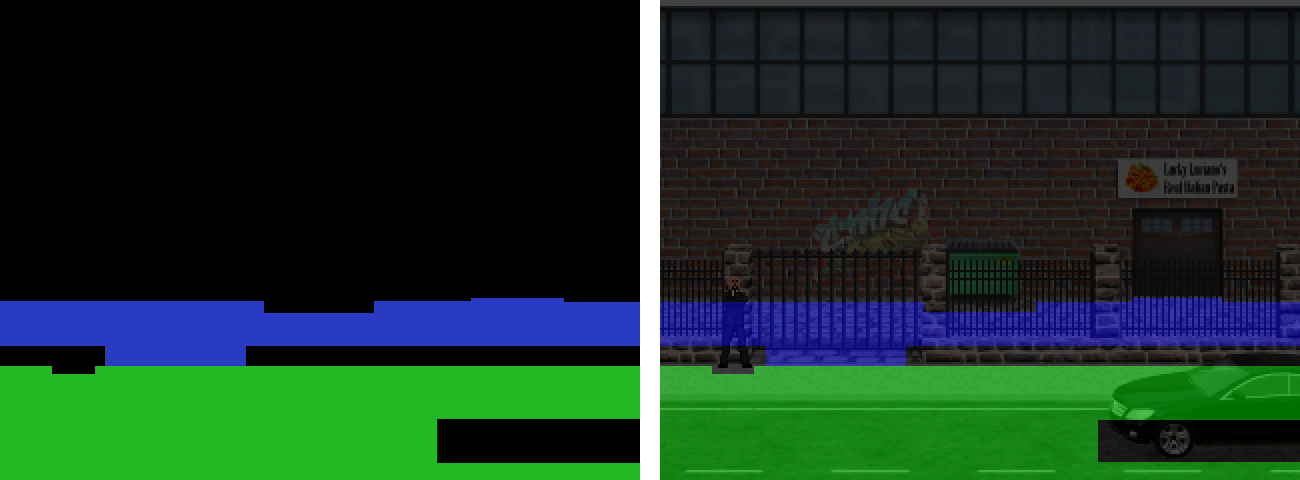
\includegraphics[width=1.0\linewidth]{img/walkability-map2.png}
\caption{Walkability bitmap: bitmap mask (left) and mask applied on top of a scene (right). Source \cite{Shdon}.}
\label{fig:WS:Bitmap}
\end{figure}

To obtain such a bitmap, the user must use image-editing software to manually create colorful shapes that represent the accessible parts of the environment and then save the image. Additionally, modifying the bitmap is difficult and time-consuming, as it requires reopening the editing software and making manual changes. Our goal is to find a solution that can be integrated directly into the framework while keeping the experience user-friendly, something this approach does not support. 

The second option enables us to create the map in the Unity engine itself. The idea is to have one primary shape that defines the main walkable area, be it a room, a hall, or a town square. Inside that area, there can be places that are not accessible currently or indefinitely (e.g. furniture), let us call them obstacles. We can define the boundaries of the walkable area and the obstacles using polygons, as seen in Figure \ref{fig:WS:Poly}. One such polygon can be used to outline the primary area where the user walks around, while additional polygons can be viewed as obstacles that the player must avoid. This implementation is examined in detail in the articles by Mic Uurloon \cite{Uurloon1}\cite{Uurloon2}.

The main advantage of this approach is the ability of the user of the framework to modify the shapes on the fly whenever necessary. Next, this system can be implemented directly in Unity and does not require any other software to set it up. For these reasons, we decided to go with this solution.

\begin{figure}[H]
\centering
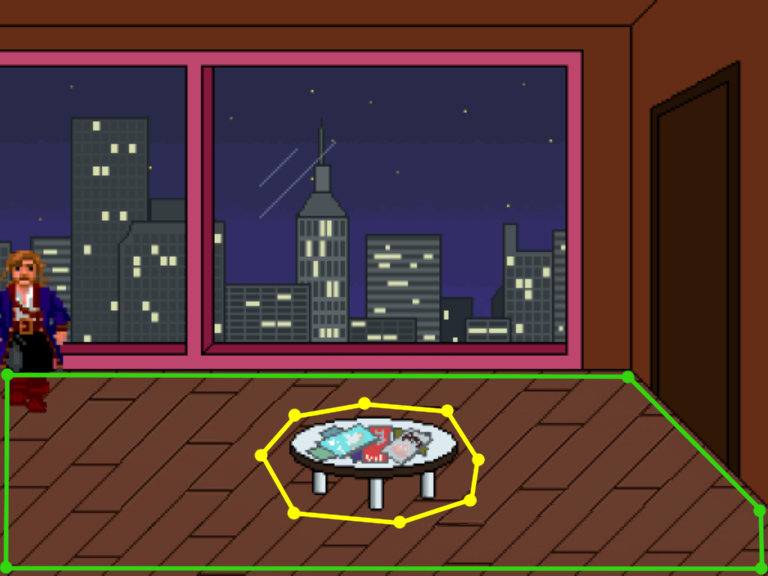
\includegraphics[width=.8\linewidth]{img/WS-polygons4.png}
\caption{Polygonal map: the room as the main walkable area (green) and the table as an obstacle (yellow). Source \cite{Uurloon1}.}
\label{fig:WS:Poly}
\end{figure}

\subsection{Pathfinding}
A crucial part of character movement is the ability to find a path to the goal. Objects typically get there by taking the shortest route possible. This makes sense in point-and-click adventure games, as player input is intentional and direct: clicking on a location implies that the character should move there efficiently, without unnecessary detours. The problem of finding the shortest path is a well-studied field in computer science, with several established algorithms designed to solve it. 

\subsubsection{Weighted Graph}
Polygons only serve as a visual representation of the walkable area to the framework users, and essentially this is everything they need to care about. However, to enable algorithms like pathfinding to operate effectively, the walkable area must also be represented in a form suitable for computation. Specifically, if we want to determine the shortest path to a destination, we need a way to calculate the distances between the points—without this, identifying the optimal route would be impossible. A weighted graph provides an ideal structure for this purpose. It consists of nodes connected by edges, each assigned a non-negative value representing the distance between them. That said, generating a graph that includes every possible node and edge would be both inefficient and impractical. So let us set up some rules that we need to follow:

\begin{enumerate}[label=\color{purple}\textbf{R{\arabic*}}]
  \item \label{analysis:concave} In the main polygon, every concave vertex (a vertex with an interior angle greater than 180°) is a node.
  \item \label{analysis:convex} In the obstacle polygons, every convex vertex (a vertex with an interior angle less than 180°) is a node.
  \item \label{analysis:start} The position of the character (start position) is a node.
  \item \label{analysis:end} The end position (e.g. the mouse cursor) is a node.
  \item \label{analysis:LOS} For each two nodes, we create an edge if they are in line of sight (a straight line from a node to another node inside the polygon without crossing an edge of any polygon). 
\end{enumerate}

According to Rule \ref{analysis:concave}, a node is included based on type of the vertex of the corresponding polygon. In basic shapes like triangles, rectangles, and squares, any two points can be connected by a straight line without encountering obstacles. However, if the walkable area is concave (containing one or more concave verices), some vertices point inward, creating obstructions that block direct visibility between points, as depicted in Figure \ref{fig:Polygons}. To account for these obstructions, a node is added to the graph only if its corresponding vertex is concave. On the other hand, convex vertices are excluded as they do not create such obstructions.

\begin{figure}[H]
\centering
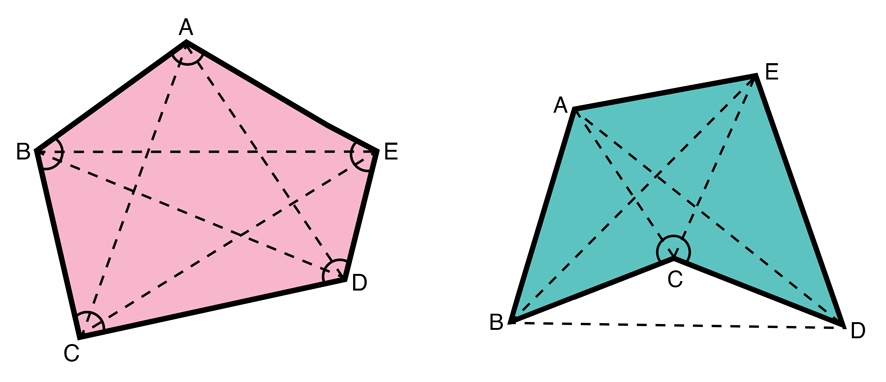
\includegraphics[width=.8\linewidth]{img/polygons.png}
\caption{Convex (left) and concave (right) polygons. Source \cite{Polygons}.}
\label{fig:Polygons}
\end{figure}

To determine which vertices are convex, we can iterate through them one by one and check the angle formed by the lines from the previous and next vertices to the current one. We do that by calculating the cross product, as seen in Algorithm \ref{alg:IsVertexConcave}.

\algrenewcommand\algorithmicrequire{\textbf{Input:}}
\algrenewcommand\algorithmicensure{\textbf{Output:}}
\renewcommand{\alglinenumber}[1]{#1.}  % Change numbering from "1:" to "1."
\begin{algorithm}[H]
\caption{Check if a Vertex is Concave}\label{alg:IsVertexConcave}
\begin{algorithmic}[1]
\Require Array of vertices $vertices$, index of vertex $vertex$
\Ensure \textbf{true} if the vertex is concave, \textbf{false} otherwise
\Statex
\Function{IsVertexConcave}{$vertices, vertex$}
    \State $current \gets vertices[vertex]$
    \State $next \gets vertices[(vertex + 1) \bmod \Call{Length}{vertices}]$
    \If{$vertex = 0$}
        \State $previous \gets vertices[\Call{Length}{vertices} - 1]$
    \Else
        \State $previous \gets vertices[vertex - 1]$
    \EndIf
    \State $left \gets$ \Call{Vector}{$current.x - previous.x,\ current.y - previous.y$}
    \State $right \gets$ \Call{Vector}{$next.x - current.x,\ next.y - current.y$}
    \State $cross \gets (left.x \cdot right.y) - (left.y \cdot right.x)$
    \State \Return $cross < 0$
\EndFunction
\end{algorithmic}
\end{algorithm}

However, this method can produce incorrect results if the vertex order is not handled carefully. Reversing the order of the vertices results in the opposite angle, which may misclassify the convex and concave points (see Figure \ref{fig:Clock}). The Algorithm \ref{alg:IsVertexConcave} works only in the case that the vertices of a polygon are ordered clockwise. To avoid getting the wrong result, we must also check that the vertices are ordered clockwise or counter-clockwise. This can be done using the Algorithm \ref{alg:IsOrientationClockwise}.
The algorithm essentially calculates a signed value based on the positions of consecutive vertices. It does this by summing the expression $(b.x-a.x)\cdot(b.y+a.y)$ for each edge, where $a$ and $b$ are adjacent vertices. A positive result indicates a clockwise orientation, while a negative result indicates counter-clockwise.

\begin{figure}[H]
\centering
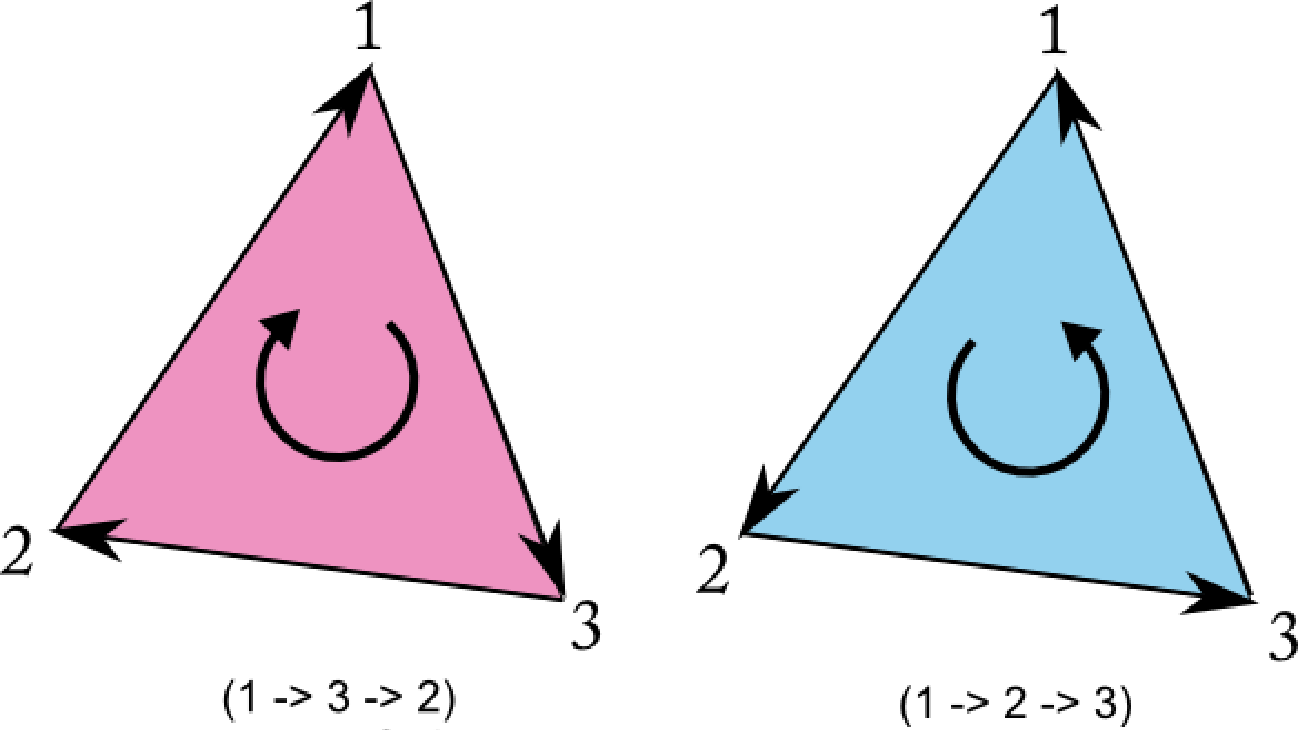
\includegraphics[width=.6\linewidth]{img/clock.png}
\caption{Clockwise (left) and counter-clockwise (right) polygons. Source \cite{Clock}.}
\label{fig:Clock}
\end{figure}

\begin{algorithm}[H]
\caption{Check if Polygon Orientation is Clockwise}\label{alg:IsOrientationClockwise}
\begin{algorithmic}[1]
\Require Array of vertices $vertices$
\Ensure \textbf{true} if orientation is clockwise, \textbf{false} otherwise
\Statex
\Function{IsOrientationClockwise}{$vertices$}
    \State $sum \gets 0$
    \For{$i \gets 0$ to $\Call{Length}{vertices} - 1$}
        \State $a \gets vertices[i]$
        \State $b \gets vertices[(i + 1) \bmod \Call{Length}{vertices}]$
        \State $sum \gets sum + (b.x - a.x) \cdot (b.y + a.y)$
    \EndFor
    \State \Return $sum > 0$
\EndFunction
\end{algorithmic}
\end{algorithm}

The next rule \ref{analysis:convex} tells us that the situation is reversed for obstacles (meaning non-main polygons) as we do not want to stay inside these obstacles but on the outside. Since we need to go around them, in this case we include convex vertices instead of concave ones. Here, the concave vertices do not stand in the way of two points, but the convex ones do. 

When it comes to the starting and ending positions (typically those of the main character and the mouse cursor), we need to include them as well. Because our primary aim is to find a path between them in the graph, the Rules \ref{analysis:start} and \ref{analysis:end} are necessary for this purpose.

Finally, in terms of edges, an edge is included in the graph only if the two nodes that form it are within each other's line of sight, as mentioned in Rule \ref{analysis:LOS}. If other edges were included, we would get edges that run through obstacles and outside of the main walkable area, which is definitely not what we want. This is why we need to do a check of visibility. The Algorithm \ref{alg:InLineOfSight} depicts the process of check if two nodes are in line of sight. \todo{finish this}

\begin{algorithm}
\caption{Check Line of Sight Between Two Points}\label{alg:InLineOfSight}
\begin{algorithmic}[1]
\Require Start point \texttt{start}, End point \texttt{end}, List of polygons \texttt{polygons}
\Ensure \textbf{true} if \texttt{start} and \texttt{end} are in line of sight, \textbf{false} otherwise
\Statex
\Function{InLineOfSight}{start, end}
    \State $\epsilon \gets 0.5$
    \If{not polygons[0].pointInside(start) or not polygons[0].pointInside(end)}
        \State \Return \textbf{false}
    \EndIf
    \If{Length(Subtract(start, end)) < epsilon}
        \State \Return \textbf{false}
    \EndIf
    \State inSight $\gets$ \textbf{true}
    \ForAll{polygon in polygons}
        \For{$i \gets 0$ to Length(polygon.vertices) $-1$}
            \State $v1 \gets$ polygon.vertices[$i$]
            \State $v2 \gets$ polygon.vertices[$(i+1) \bmod$ Length(polygon.vertices)]
            \If{LineSegmentsCross(start, end, v1, v2)}
                \If{distanceToSegment(start.x, start.y, v1.x, v1.y, v2.x, v2.y) > 0.5 and distanceToSegment(end.x, end.y, v1.x, v1.y, v2.x, v2.y) > 0.5}
                    \State \Return \textbf{false} 
                \EndIf
            \EndIf
        \EndFor
    \EndFor
    \State $v \gets$ Add(start, end)
    \State $mid \gets$ Vector($v.x / 2$, $v.y / 2$)
    \State $inside \gets$ polygons[0].pointInside(mid)
    \For{$i \gets 1$ to Length(polygons) $-1$}
        \If{polygons[$i$].pointInside(mid, false)}
            \State $inside \gets$ \textbf{false}
        \EndIf
    \EndFor
    \State \Return $inside$
\EndFunction
\end{algorithmic}
\end{algorithm}

By combining all of these Rules \ref{analysis:concave}--\ref{analysis:LOS}, we get a graph showing possible ways to get between points (see Figure \ref{fig:Graph}). This entire algorithm for creating a graph from polygons was adapted from the articles by Mic Uurloon. Details about this method together with more interactive examples explaining how the algorithm works can be found in his articles Part 1 \cite{Uurloon1} and Part 2 \cite{Uurloon2}.

\begin{figure}[H]
\centering
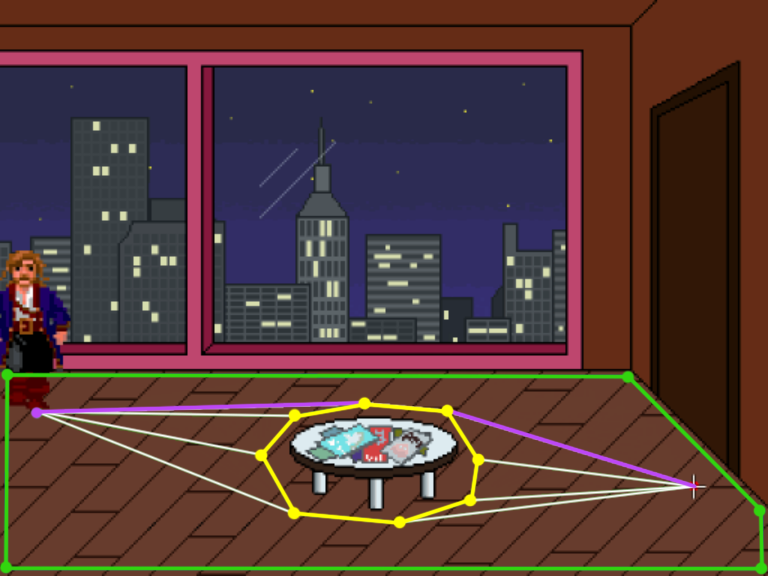
\includegraphics[width=.8\linewidth]{img/WS-polygons3.png}
\caption{Graph: Walkable area consisting of polygons (green and yellow) and a graph (white) with a possible path (violet). Source \cite{Uurloon1}.}
\label{fig:Graph}
\end{figure}

\subsubsection{A* algorithm}
When it comes to the algorithms themselves, we aim to find one that would reliably and efficiently determine the shortest path between two points in a 2D space while maintaining reasonable performance. A* is a strong candidate for this purpose—it is a graph traversal and pathfinding algorithm widely used in the games because of its efficiency. A key component of the A* algorithm is the heuristic function which estimates the cost of the cheapest path to the goal. If the function never overestimates it, A* is guaranteed to return one of the shortest paths from start to goal. For the purpose of free character movement on a 2D plane, the Euclidean distance was chosen as a heuristic function. It is well-suited for point-and-click adventure games, where characters can move freely in any direction, making straight-line distance a natural and accurate estimate of travel cost.  It can be calculated from the Cartesian coordinates of the points while also applying the Pythagorean theorem:

\[
d = \sqrt{(x_2 - x_1)^2 + (y_2 - y_1)^2}
\]

\section{Depth Simulation}
As we have specified in Requirements \ref{intro:req:scale} and \ref{intro:req:layers}, we want to simulate the feeling of a 3D space.

\subsection{Scaling}
\label{analysis:depth:scaling}
Firstly, we will look closely at character scaling. There are a number of ways we can achieve this. An option would be to do so by only looking at the Y coordinates. This way, we can set boundaries for the minimum and the maximum scale of the moving object in the given area, and then, based on the distance from those boundaries, set the appropriate value. This approach is very simple, which is both its advantage and its disadvantage. Although it is easy to implement, it is not possible to achieve more complex scenes in which a character's sprite scales dynamically independently of the Y coordinates. A similar problem would arise with only considering the X coordinates.

Another option is to keep additional information on the scaling inside the vertices of polygons that make up the walkable map. By doing so, we could calculate the scaling factor based on the distance from each node with a floating number representing the scaling. This approach is a bit more complicated, but still simple to implement. An advantage is the fact that the developer could have a free range on the exact details of the area. However, modifying the scales is not that easy because it is necessary to go through the necessary nodes and change the factor by hand.

Finally, it is possible to use a bitmap and map the alpha value of each pixel to a scaling factor. This would be very precise, as the developer can set it up exactly as they wish. However, we again come across the problem we discussed in Section \ref{analysis:walkableMap} where we made it clear that we prefer to implement features that can be simply modified inside Unity.

From these three approaches only two seem to be doable entirely inside the framework: Y scaling (optionally X scaling) and custom vertices scaling. We aim to implement both of them in the hopes of offering a wide variety of options to developers.

\subsection{Layering}
Next, let us examine the layering. Our aim is to dynamically adjust the visibility of objects, as seen in Figure \ref{fig:Layers}. Because we are working with a 2D space, we have to do a bit more work determining in what order the sprites of objects should be displayed. Fortunately, it is very simple since all we need is to look at the Y coordinates. If object A has a smaller Y coordinate than object B, it means that A should be drawn on top of B. This is not complicated, but also not trivial, since it would be necessary to perform this check between each two objects in the scene. Lucky for us, Unity offers tools for 2D renderer sorting \cite{Unity-sorting} and can therefore take care of this problem for us. What we are looking for is the Custom Axis sort mode \cite{Unity-customAxis} in Graphics section under the Project Settings window. Details on the setup with a couple more modifications to make it just right can be found online in the Sunny Valley Studio article \cite{Piotr} . 

\begin{figure}[H]
\centering
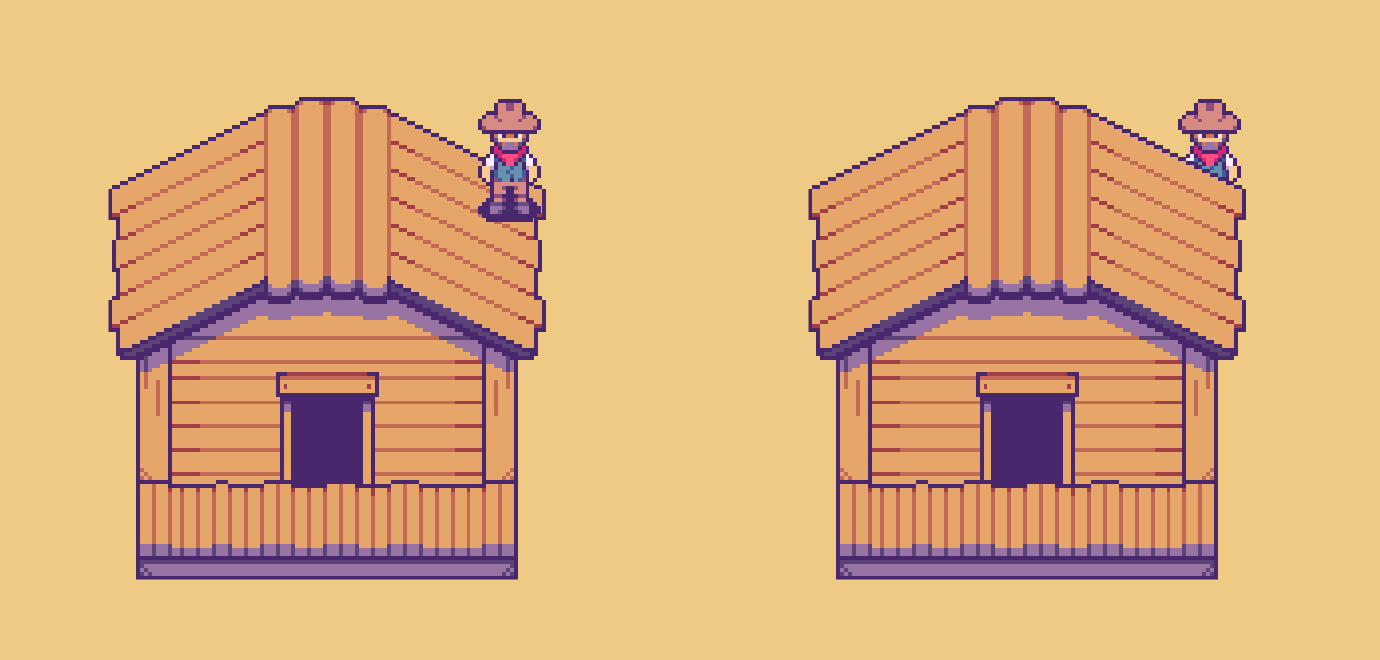
\includegraphics[width=.8\linewidth]{img/layers.png}
\caption{Wrong (left) and correct (right) 2D layer ordering. Source \cite{Piotr}.}
\label{fig:Layers}
\end{figure}

\section{Inventory System}


\section{Dialogue System}


